\documentclass[11pt,a4paper,sans]{moderncv} 
\moderncvstyle{banking}
\moderncvcolor{blue}
\usepackage[scale=0.75]{geometry}

% Información personal
\name{Jose Alejandro}{Carrillo Mora}
\phone[mobile]{+57~(301)~788~7149}
\email{alejo-carrillo@outlook.com}

% Foto
\begin{flushright}
  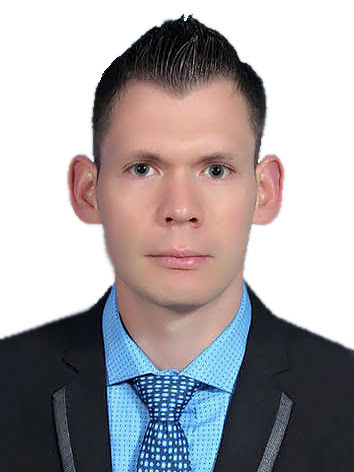
\includegraphics[width=3cm]{foto.jpg}
\end{flushright}

\begin{document}
\makecvtitle

% PERFIL PROFESIONAL
\section{Perfil Profesional}
\cvitem{}{Administrador de Empresas, con experiencia en áreas de atención al cliente, comerciales y administrativas, manejo de herramientas ofimáticas, bases de datos y herramientas web. Soy una persona responsable, con excelente actitud, creativo, organizado, con habilidad de trabajo en equipo y excelentes relaciones interpersonales. Me apasiona viajar, la música, el microfútbol, aprender nuevos idiomas y los deportes extremos.}


% FORMACIÓN ACADÉMICA
\section{Formación Académica}
\cventry{2023 -- en curso}{Maestria en análisis de datos}{Universidad Central}{Bogotá, Colombia}{}{}

\cventry{2015 -- 2019}{Administrador de Empresas}{Corporación Universitaria Minuto de Dios}{Bogotá, Colombia}{}{}
\cventry{2019}{Diplomado en Tributaria}{Corporación Universitaria Minuto de Dios}{Bogotá, Colombia}{}{}
\cventry{2003 -- 2011}{Bachiller académico- Énfasis en gestión de empresas}

% TRAYECTORIA LABORAL
\section{Trayectoria Laboral}
\cventry{Jun 2021 -- actual}{Analista de Requerimientos Legales}{Claro Colombia}{Bogotá, Colombia}{}{Funciones realizadas: Gestión de servicios móviles, Tester, atención a clientes internos y externos, gestión de PQRS y manejo de bases de datos, elaboración de informes e indicadores.}{} \vspace{2mm}
\cventry{May 2018 -- Jun 2021}{Asesor Gestión PQRS}{Claro Colombia}{Bogotá, Colombia}{}{Funciones realizadas: Gestión de PQRS y manejo de bases de datos. Logros: Ascenso laboral.}\vspace{2mm}
\cventry{Sep 2016 -- Abr 2018}{Auxiliar de Activaciones y convenios empresariales}{Droguerías y Farmacias Cruz Verde S.A.S}{Bogotá, Colombia}{}{}{Funciones realizadas: Atención al cliente interno y externo, atención de proveedores, manejo de inventario, elaboración de informes e indicadores, manejo de herramientas ofimáticas, manejo de caja POS y abastecimiento de máquinas Vending. Logros: Implementación y ejecución de la primera droguería móvil y de máquinas Vending de medicamentos.}

% FORMACIÓN COMPLEMENTARIA

\section{Formación complementaria}
\cventry{2018 -- en curso}{Curso de Desarrollador Web}{Google}{Bogotá, Colombia}{}{}
\cventry{2018 -- en curso}{Curso de CRM}{Senal}{Bogotá, Colombia}{}{}
\cventry{2018 -- en curso}{Curso de Desarrollo de Apps Móviles}{Google}{Bogotá, Colombia}{}{}
\cventry{2018 -- en curso}{Curso de Cloud Computing}{Google}{Bogotá, Colombia}{}{}
\end{document}
